\documentclass[12pt, oneside]{book}
 
\usepackage{graphicx}
\usepackage{hyperref}
\graphicspath{{images/}}
\begin{document}
 
%titlepage
\thispagestyle{empty}
\begin{center}
\begin{minipage}{0.75\linewidth}
    \centering
%University logo
    
\includegraphics{UPlogo}
    \rule{0\linewidth}{0.15\linewidth}\par

%Thesis title
    {\uppercase{\Large Functional Requirements\par}}
   	{\uppercase{\Large cos 301 group 2 b \par}}
    \vspace{1cm}
%Author's name
    {\normalsize Byron Dinkelmann u11057638\par}
    {\normalsize Johan van Rooyen u11205131\par}
    {\normalsize Mandla Mhlongo u29630135\par}
    {\normalsize Ryno Pierce u12003922\par}
    {\normalsize Sylvester Mpungane u11241617\par}
    {\normalsize Molefe Molefe u12260429\par}
    {\normalsize Taariq Ghoord u10132806\par}
    {\normalsize Timothy Snayers u13397134\par}
    \vspace{1cm}
    
    \hyperref[https://github.com/ByronDinkelmann/COS-301-Group-2-b.git]{Github}\par
    \vspace{1cm}
%Date
    {\Large February 2015}
\end{minipage}
\end{center}
\clearpage

\tableofcontents
\newpage

\section{Introduction}
This document outlines the functional requirements of "The Computer Science Education Didactic and Applications Research"(CSEDAR) registered research project called "The use of Online Discussion in Teaching"(TODT). This document describes the "Buzz" system to be developed and gives insight to how to achieve this implementation for those implementing it. 
\section{Vision}
The research projects aim is to find ways to enhance and improve the learning of students with the use of online discussion. This online forum "Buzz" will become part of the Computer Science websites modules, creating an online space for discussion for each or where relevant. Where students, teaching assistants and lecturers can engage in activities
related to learning the content of the specific module while applying game concepts to motivate students to increase the quality of their participation and consequently experience deeper learning of the course content. 
\section{Background}
The reason for this research project is the problem of engaging an extremely large number of first year students within The University of Pretoria, specifically the Computer Science Department students. Currently available tools for discussion forums lead to the problems that are hampering positive engagement of teaching staff and students. These problems consist of inexperienced users, unorganized content and low levels of excitement.
To combat these problems the "Buzz" system intends to have the basic functionality of online forums, have automated feedback on common mistakes, have a Game-like presentation and have automated structuring.

The University of Pretoria have the opportunity to teach the COS301 "Software Engineering" students while being able to improve current systems of online discussion which can be extended to benefit all students in the future. 

The research project gives the students of COS301 "Software Engineering" an opportunity to learn form the experiences of designing, creating and developing this system, which include learning to work with colleagues, creating documentation, simplifying and improving the communication of lectures and students through a structured forum, using online systems for group work and the basic process of how software is designed, created and developed in business to name but a few.
\section{Functional Requirements and application design}

\subsection{Purpose}
\begin{enumerate}
 \item{CRUD}: To create posts on the buzz system so that users in the system can share relevant information with one another and communicate. To allow registered users and non registered users such as guests to view posts created by users of the buzz system. To allow users to update posts of which they control. To allow users to delete their own posts or to allow users with sufficient status level to delete other posts based on certain factors about that specific post.
 \\
\item{Message Restrictions}: To restrict users to length, content and positioning of posts based on the users status level. 
\\
 \item{Message Tracker}: To mark posts for each registered user so that they can keep track of which posts they have read and which users have read certain posts.
\\

 
\end{enumerate}

\subsection{Use case prioritization}
\subsubsection{CRUD}
Critical
\subsubsection{Message Restrictions}
Critical
\subsubsection{Message Read Tracker}
Important
\subsection{Use case/Service contracts}
\subsubsection{CRUD}
\begin{enumerate}
 \item Pre-conditions for CRUD: The buzz system needs to be available and a connection to the buzz system possible. 
\end{enumerate}
\subsubsection{CRUD-Create}
\begin{enumerate}
 \item Pre-conditions: For a user to create posts they need to be registered of the buzz system. The user must be logged in to the buzz system.
 \\
 \item Post-conditions: Posts will succeed to be created and will appear in the buzz system where posted.
  \\
 \item Request and Result Data Structures: 
\end{enumerate}

\subsubsection{CRUD-Read}
\begin{enumerate}
 \item Pre-conditions: Posts must be present to be read.
 \\
 \item Post-conditions: Once a post has been viewed by a logged in registered user, the post should be marked as read for that specific user.
  \\
 \item Request and Result Data Structures:
\end{enumerate}

\subsubsection{CRUD-Update}
\begin{enumerate}
 \item Pre-conditions:  For a user to update posts they need to be registered of the buzz system. The user must be logged in to the buzz system. The user must be the owner of the post.
 \\
 \item Post-conditions: Post will be updated and shown on the buzz system to be updated.
   \\
 \item Request and Result Data Structures:
\end{enumerate}

\subsubsection{CRUD-Delete}
\begin{enumerate}
 \item Pre-conditions:  For a user to delete posts they need to be registered of the buzz system. The user must be logged in to the buzz system. The user must be the owner of the post unless a user with status level "x" views the post to be unfit. The post needs to exist for it to be deleted.
 \\
 \item Post-conditions: Post successfully deleted will be hidden from the other users and buzz system and archived.Posts will never be physically deleted from the system itself.
   \\
 \item Request and Result Data Structures:
\end{enumerate}

\subsubsection{Message Restrictions}
\begin{enumerate}
 \item Pre-conditions:  User must be registered on the buzz system. The buzz system needs to be available and a connection to the buzz system possible. The user must be logged in to the buzz system. User must be able to create posts. Length and content of posts must be specified by the buzz system of which the user is registered. Must have levels of posts.
 
 \item Post-conditions: Post will be created and shown on the buzz system. Correct length and content of posts if buzz system is configured correctly.
   \\
 \item Request and Result Data Structures:
\end{enumerate}

\subsubsection{Message Read Tracker}
\begin{enumerate}
 \item Pre-conditions:  User must be registered on the buzz system. The user must be logged in to the buzz system. Messages must exist to be read, marked as unread and must be seen as read by other users.
 \\
 \item Post-conditions: Post is marked as unread.Post is marked when read and seen to be read on the buzz system.
   \\
 \item Request and Result Data Structures:
\end{enumerate}


\subsection{Required functionality}
\subsection{Process specifications}
\subsection{Domain Model}
\section{Open Issues}


\section{Searching and Filtering}
\subsection{Description:}
Users will make use of such functionality to locate hard to find information like specific phrases within posts or category headings. The user will also use this functionality be able to sieve through the forum to track down other users and/or topics.  
\subsection{Actors:} 
Active forum members, administrators, evaluators will be the most common users of this functionality. Guests and other passive forum members will be the uncommon users.
\subsection{Preconditions:} 
Guests are able to search/filter but a limited search results would be imposed depending on the search criteria. Higher level users (forum members and ranked forum members) would have less restricted search capability based on the user ranking system. Super users (Administrators and Evaluators). \subsection{Basic Flow:} 
The actor will type in the search term and select advanced criteria (optional, less restricted based on actor rank). The search is processed, this involves database querying and third party search engines. Results displayed in a categorical fashion. Categories (posts, subjects, topics, members etc.) from the results are scanned by the actor. A Result selection leads the actor directly to the selected results origin. A search rating mechanism would occasionally ask for a search rating.  
\subsection{Alternative Flows:} 
For uncommon users the search is less intensive and restricted thus shallow search processing will occur. Security questions would have to be answered occasionally. The browser checked cached search results. The results would still be presented in a categorical form, but would obviously omit restricted results. 
\subsection{Exception Flows:} 
Unintelligible or foreign language search’ would be severely limited. However technical jargon in search terms will be accommodated to an extent. Search results with restricted content would require user login to display.
\subsection{Post Conditions:} 
Search results are directly linked to their displayed source. A search/filter with no hits will display related content and help for bettering the search.
\subsection{User Case Diagram}
\begin{center}
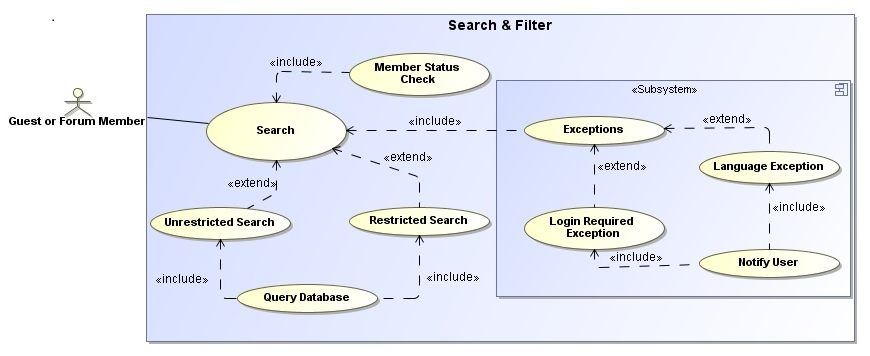
\includegraphics[scale=0.5]{SearchAndFilter.png}
\end{center}
\section{Post Evaluation and Voting}
\subsection{Description:} 
Users would occasionally be approached to assess other users and their posts on the forum, users can also willingly rate posts or topics they have read through. Evaluation criteria would include the integrity of the information in posts and the posters rank and forum activity.
\subsection{Actors:} 
Only forum members can participate in post evaluation and voting. There are possible exceptions like security cleared +1 members (temporary members linked to a current forum member) or forum guests that are identifiable experts   on a topic/subject. 
\subsection{Preconditions:} 
The actor must be a forum member or have qualified to vote based on the above mentioned exceptions. The voter must be of a certain rank to access advanced voting functionality. The voter must be clear of any bans. 
\subsection{Basic Flow:} 
The user will click on the voting mechanism linked to the post. The voting window will appear and the voters profile and history will be checked. The voting will then commence and allow for more or less voting capabilities based on the voters details. The vote will be submitted and the optional evaluation (for ranked voters only) will be sent to the post owner and displayed alongside the post.
\subsection{Alternative Flows:} 
The exception user will place a vote on a post. The linked forum member will be informed of this action. The vote and evaluation will be submitted upon the forum members’ approval. 
\subsection{Exception Flows:} 
The user has been banned from voting and is denied voting and evaluation rights until he/she obtains an acceptable rank or is unbanned by the forum administrator.
\subsection{Post Conditions:} 
The voter and vote receivers’ profiles are updated and rank re-evaluated. The vote/evaluation on the post is updated instantly. 
\subsection{User Case Diagram}
\begin{center}
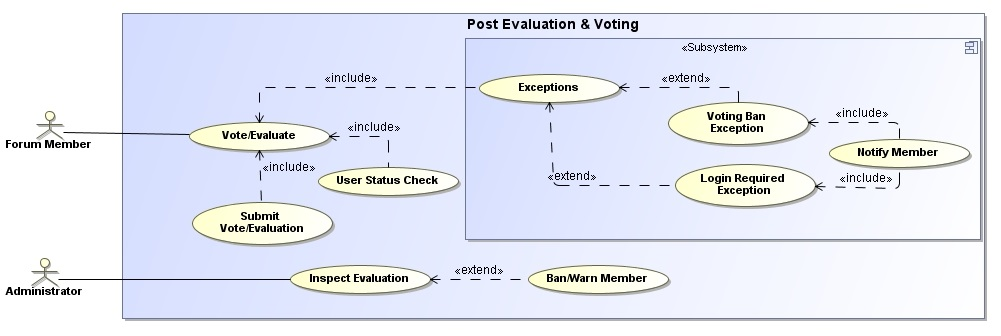
\includegraphics[scale=0.4]{PostVoteAndEvaluation.png}
\end{center}

\section{Changing User Status}
\subsection{Description}
The Buzz system will automatically rank users of the system based on their participation. A user's  reputation (status) will be affected by the user's participation points on Buzz system, it can either grow or be negatively affected depending on the user's participation marks.   
\subsection{Actors}
This functionality will be automatically triggered by the Buzz system each time a user's participation is evaluated.
\subsection{Preconditions}
The user needs to earn new participation points (positive or negative).
\subsection{Post Conditions}
The user's status will either have changed or remained the same depending on which status the participation points correspond with.
\subsection{Use Case Diagram}

\section{Integrating System with any Specified Host}
\subsection{Description}
The system should have the ability to be hosted by any site that it specified on setup.
\subsection{Actors}
The administrator of the host site is the only user that can use this functionality.
\subsection{Preconditions}
The user must be the site administrator and the host site specified must be a valid site.
\subsection{Post Conditions}
The system should be integrated on the site.
\subsection{Use Case Diagram} 
\end{document}